\begin{figure*}

\centering

\begin{subfigure}{0.31\linewidth}
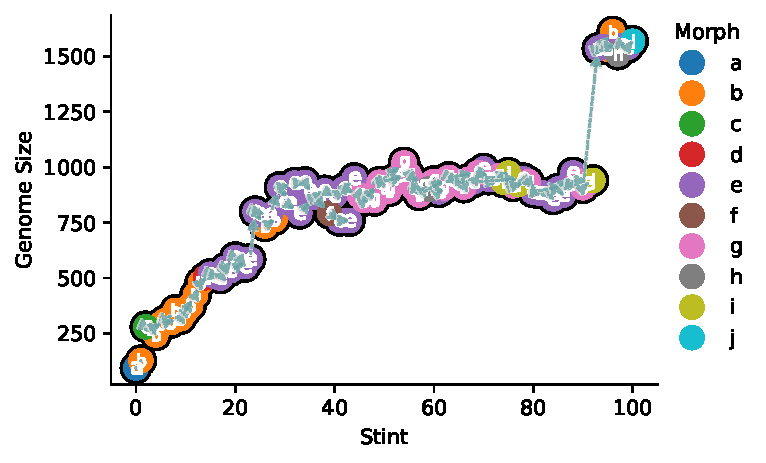
\includegraphics[width=\linewidth, clip, trim={0 0 1.6cm 0}]{binder-2025-08-26-dotfig/binder/teeplots/2025-08-26-dotfig/bucket=prq49+cat=morph+endeavor=16+transform=filter-Series-16005+viz=letterscatter+x=stint+y=num-instructions+ext=.pdf}
\end{subfigure}
~
\begin{subfigure}{0.29\linewidth}
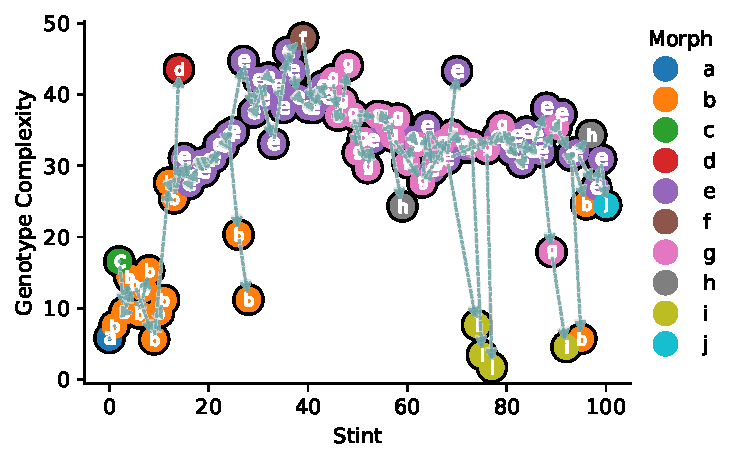
\includegraphics[width=\linewidth, clip, trim={0 0 1.6cm 0}]{binder-2025-08-26-dotfig/binder/teeplots/2025-08-26-dotfig/bucket=prq49+cat=morph+endeavor=16+transform=filter-Series-16005+viz=letterscatter+x=stint+y=critical-fitness-complexity+ext=.pdf}
\end{subfigure}
~
\begin{subfigure}{0.35\linewidth}
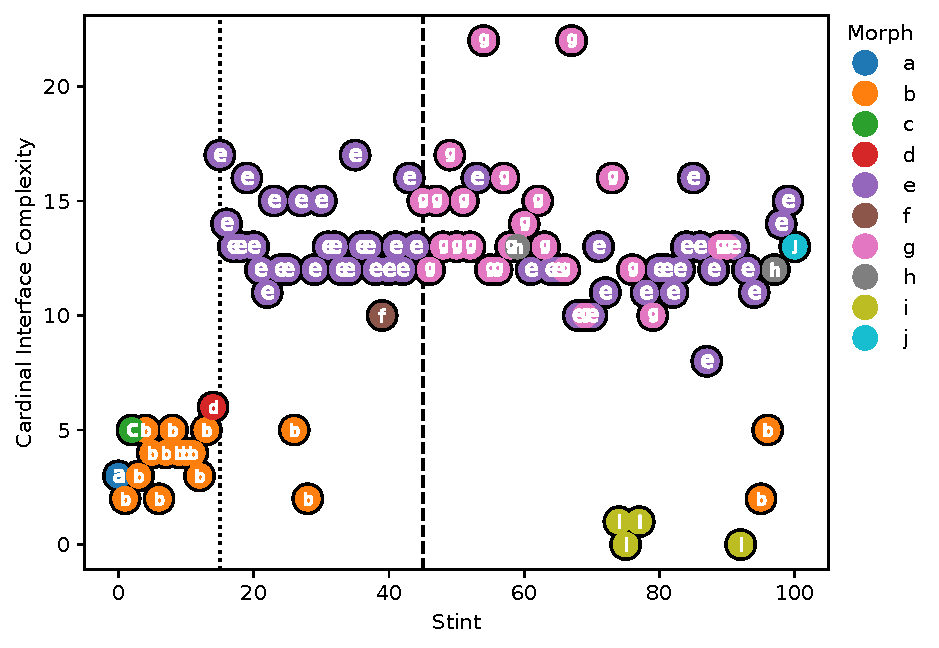
\includegraphics[width=\linewidth, clip, trim={0 0 0 0}]{binder-2025-08-26-dotfig/binder/teeplots/2025-08-26-dotfig/bucket=prq49+cat=morph+endeavor=16+transform=filter-Series-16005+viz=letterscatter+x=stint+y=cardinal-interface-complexity+ext=.pdf}
\end{subfigure}%

\begin{minipage}{\linewidth}
\centering
\begin{minipage}[t]{0.31\linewidth}
\subcaption{\footnotesize
genome size
}
\label{fig:complexity:size}
\end{minipage}
~
\begin{minipage}[t]{0.29\linewidth}
\subcaption{\footnotesize
genetic complexity
}
\label{fig:complexity:genetic}
\end{minipage}
~
\begin{minipage}[t]{0.35\linewidth}
\subcaption{\footnotesize
phenotypic complexity
}
\label{fig:complexity:phenotypic}
\end{minipage}
\end{minipage}

\caption{%
\textbf{Genome content and complexity.}
\footnotesize
Genome size (panel \ref{fig:complexity:size}) is the total number of genome sites.
Genetic complexity (panel \ref{fig:complexity:genetic}) is the count of genome sites with detectable fitness loss in knockout trials.
Phenotype complexity (panel \ref{fig:complexity:phenotypic}) is a count of distinct input/output interfaces between cell and environment/neighbors with detectable fitness loss in knockout trials.
Color coding corresponds to morphology categorization (Table \ref{tab:morph_by_stint}).
Measures are with respect to sampled focal strain specimen at each stint.
Arrows indicate estimated phylogenetic relationships.
}
\label{fig:complexity}
\end{figure*}
